\chapter{Model}
This chapter describes in detail the building that is analyzed, the purpose of the building, the technical installations and assumptions and simplifications that are made for the model used in energy simulations.

\section{Location and Climate}
The building analyzed is located in Shanghai, China. At an latitude of 31.17$^o$ N and longitude of 121.43 $^o$ E it is in the category "hot summer and cold winter zone" according to Chinese regulations. That means there is a big demand for heating in the winter months, and for cooling in the summer months. Relative humidity is high in the region and dehumidification needs to be considered. 

\begin{figure}[h!]
    \centering
    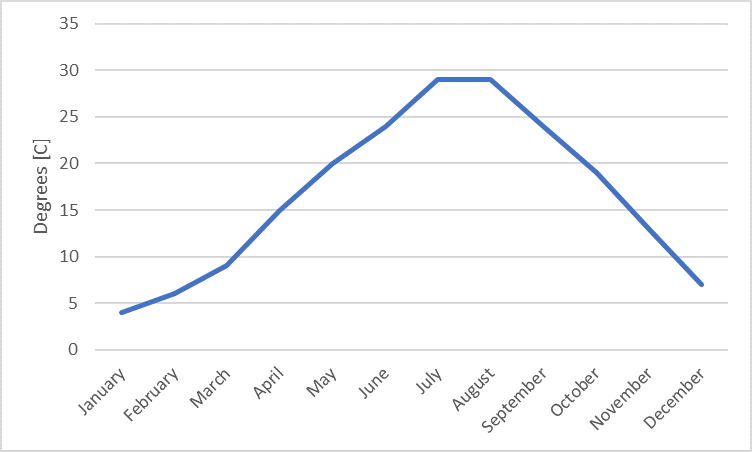
\includegraphics[scale=0.6]{vedlegg/tem.png}
    \caption{Average temperatures in Shanghai by month \cite{temp}.}
    \label{fig:temp}
\end{figure}

\subsection*{Governmental Requirements}
There are many factors influencing the energy demand of a building. For simplification the main focus is on the heat transfer coefficient or U-value of the building envelope. The authorities in China has design standards for u-values according to what climate zone the building is located, and the most relevant values is displayed in table \ref{tab:uvalue}. 

\begin{table}[h!]

    \centering
        \caption{U-value requirements for new commercial buildings in hot summer cold winter climate zone, China. \cite{uvalue}}
    \begin{tabular}{|p{1.5cm}|p{1cm}|}
         \hline
         \multicolumn{2}{|c|} {\textbf{U-value (W/m$^2$K)}} \\
         \hline
         \textbf{Roof} & 0.7 \\
         \hline
         \textbf{Wall} & 1\\
         \hline
         \textbf{Floor} & 1 \\
         \hline
         \textbf{Window} & 2.5\\
         \hline
         \textbf{Other} & 3\\
         \hline
    \end{tabular}

    \label{tab:uvalue}
\end{table}


\section{The Building}
The building is a 1 story, commercial, office building with a total of 420m$^2$. It consists of one closed office, one conference room, one open office room, one mechanical room, a break room and two restrooms. The building geometry is illustrated in figure \ref{fig:zones} where the different construction materials between interior and exterior walls can be seen.

\begin{table}[h!]
    \centering
        \caption{Caption}
    \begin{tabular}{|c|c|c|}
    \hline
    Space & Geometry & Area \\
    \hline
        Closed Office & 6m $\cdot$ 6m & 36m$^2$  \\
        \hline
        Conference Room & 6m $\cdot$ 12m & 72m$^2$  \\
    \hline
    Open Office & 10m $\cdot$ 20m + 2m $\cdot$ 2m & 204m$^2$ \\
    \hline
    Mechanical Room & 3m $\cdot$ 6m & 18m$^2$ \\
    \hline
    Break Room & 9m $\cdot$ 6m & 54m$^2$ \\
    \hline
    Restrooms & 2 $\cdot$ 3m $\cdot$ 6m & 36m$^2$ \\
    \hline
    Total & & 420m$^2$\\
    \hline
    \end{tabular}

    \label{tab:my_label}
\end{table}

\begin{figure}[h!]
    \centering
    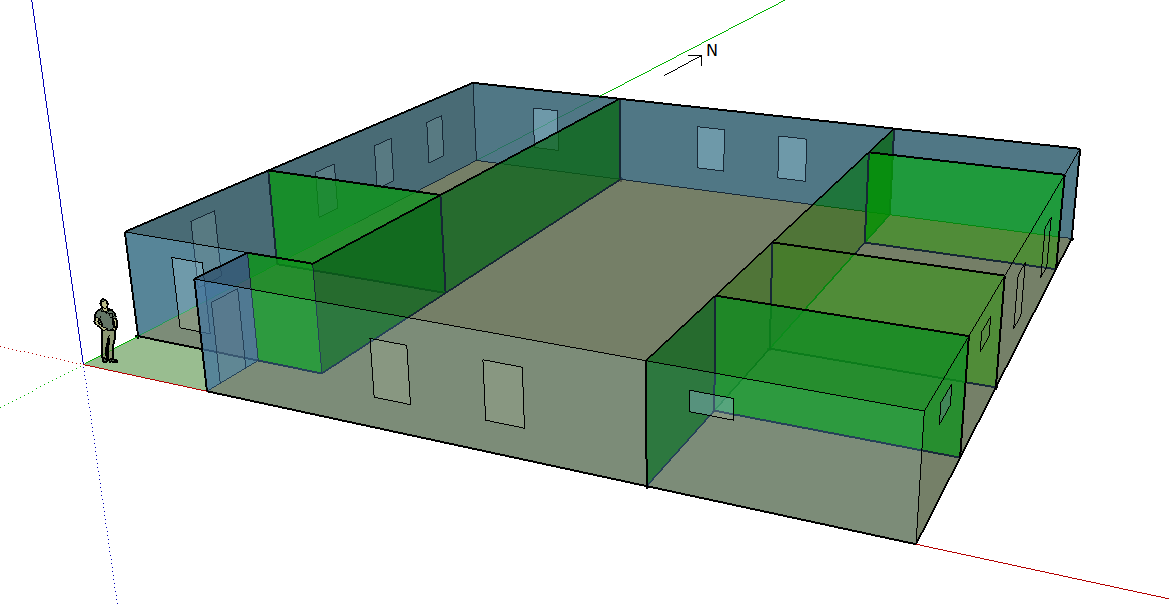
\includegraphics[scale=0.4]{vedlegg/DMozN.png}
    \caption{Building geometry}
    \label{fig:zones}
\end{figure}

\section{Building Envelope}
The U-values in the construction materials in the building envelope, simulated in EnergyPlus can be seen in table \ref{tab:Uvalue}.

\begin{table}[h!]
    \centering
        \caption{U-values, building envelope}
    \begin{tabular}{p{2cm}|p{1.8cm}|p{2cm}}
         \textbf{Surface} & \textbf{Thermal resistance} $\mathbf{[m^2}$\textbf{K/W]} & \textbf{U-value [W/} $\mathbf{m^2}$\textbf{K]} \\
         \hline
        Roof & 4.3564 & 0.2295  \\
        \hline
        External walls & 1.5106 & 0.6620 \\
         \hline
        Floor & 1.064 & 0.9397 \\
         \hline
         Windows & 0.4494 & 2.225 \\
    \end{tabular}
    \label{tab:Uvalue}
\end{table}

Comparing table \ref{tab:uvalue} and table \ref{tab:Uvalue}, the U values in the building envelope can be observed to be within Chinese governmental regulations.

\section{Thermal Zones}
The building is divided into different thermal zones according to the use of the room. The two restrooms are the only zones that are simulated based on the same criterias, but also there will two separate calculations be made.

\begin{figure}[h!]
    \centering
    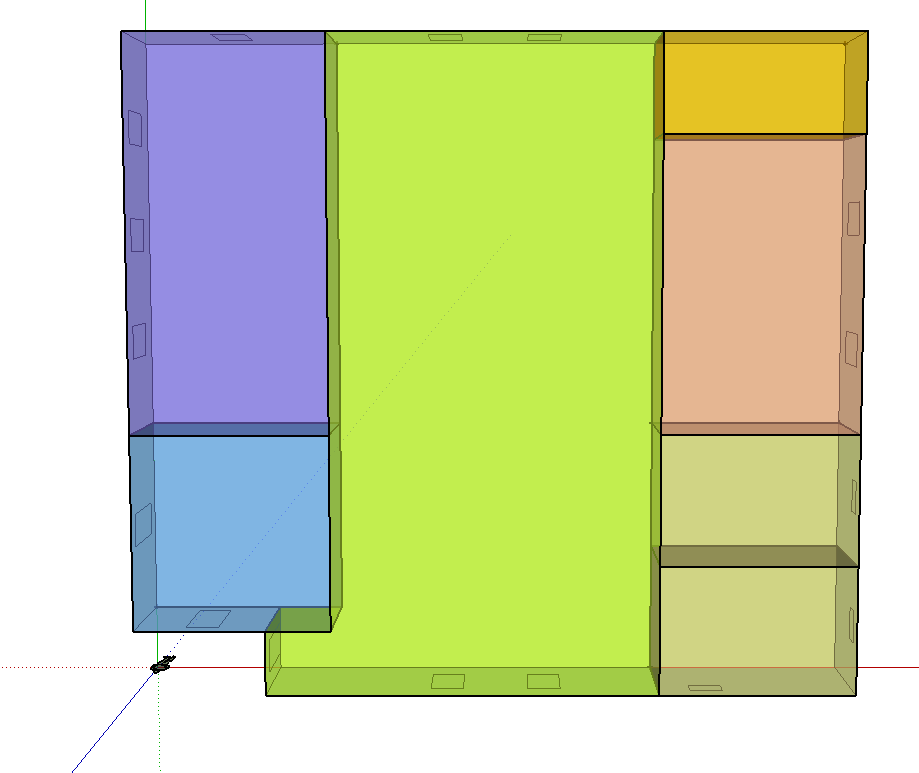
\includegraphics[scale=0.5]{vedlegg/zone.png}
    \caption{Caption}
    \label{fig:thermal}
\end{figure}

\section{HVAC}
It is assumed activity in the building between 08.00 and 16.00, with an activity level of 1.2 met. clothing level is assumed to be 1 clo all year around. Thermal comfort in the given conditions is between 22-24 degrees. 
\section{PV panels}
The roof has an area of 420m$^2$ where PV moduls will be placed

\section{Quality assurance}
\subsection{Verification}

To verify the model, certain parameters has been changed to analyze the impact on the simulation. Table \ref{tab:comp} shows the energy demand for heating and cooling at different heating and cooling setpoints. There is a lower total energy demand and peak load demand for both heating when heating setpoint temperature is 20$^o$C compared to 21$^o$C. The same accounts for total cooling demand and peak load for cooling when setpoint temperature for cooling is set to 26$^o$C, compared to 24.5$^o$C. These results is in accordance to what to expect in real life, and it is therefore a valid verification. 

\begin{table}[h!]
    \centering
        \caption{Energy demand for space heating and cooling at different setpoint temperatures}
    \begin{tabular}{|p{2.8cm}|p{1.8cm}|p{1.8cm}|}
         \hline
        & \textbf{Heating} & \textbf{Cooling} \\
        \hline
    \multicolumn{3}{|c|}{Heating setpoint 21$^O$C, cooling setpoint 24.5$^O$C} \\
    \hline
        \textbf{Total energy demand [kWh]} & 39013.6 & 24820.2 \\
        \hline
        \textbf{kWh/m$^2$} & 97.0  & 61.7 \\
        \hline
        \textbf{Peak load [kW]} & 19.9 & 37.1 \\
        \hline
    \multicolumn{3}{|c|}{Heating setpoint 20$^O$C, cooling setpoint 26$^O$C} \\
        \hline
        \textbf{Total energy demand [kWh]} & 26583.9 & 15959.7 \\
        \hline
        \textbf{kWh/m$^2$} & 63.3  & 38.0 \\
        \hline
        \textbf{Peak load [kW]} & 17.4 & 33.0 \\
        \hline
    \end{tabular}
    \label{tab:comp}
\end{table}

Table \ref{tab:com} shows simulations with different insulation thickness in the external wall. A thicker insulation thickness results in lower energy demand for heating and cooling, and a lower peak load demand. This is naturally exactly as expected and another good validation of the model. 

\begin{table}[h!]
    \centering
        \caption{Energy demand for space heating and cooling at different wall insulation thickness}
    \begin{tabular}{|p{2.8cm}|p{1.8cm}|p{1.8cm}|}
         \hline
        & \textbf{Heating} & \textbf{Cooling} \\
        \hline
    \multicolumn{3}{|c|}{External wall, insulation thickness 33.7mm} \\
        \hline
        \textbf{Total energy demand [kWh]} & 26583.9 & 15959.7 \\
        \hline
        \textbf{kWh/m$^2$} & 63.3  & 38.0 \\
        \hline
        \textbf{Peak load [kW]} & 17.4 & 33.0 \\
        \hline
    \multicolumn{3}{|c|}{External wall, insulation thickness 56.6mm} \\
        \hline
        \textbf{Total energy demand [kWh]} & 25810.4 & 15321.0 \\
        \hline
        \textbf{kWh/m$^2$} & 61.5  & 36.5 \\
        \hline
        \textbf{Peak load [kW]} & 16.9 & 32.3 \\
        \hline
    \end{tabular}
    \label{tab:com}
\end{table}

\subsection{Validation}

To validate the model, an analysis of the simulation was made to see if all design criteria was met. Table \ref{tab:valid} shows a summary of time the setpoint temperature was not met. The table indicates the temperatures was always within wanted parameters, which is a good validation that the model works exactly as it is intended to.

\begin{table}[h!]
    \centering
        \caption{Validation of operative temperature in the building}
    \begin{tabular}{|c|c|}
         \hline
        Time setpoint not met & hr  \\
         \hline
         During heating & 0.0 \\
         \hline
         During cooling & 0.0 \\
         \hline
    \end{tabular}
    \label{tab:valid}
\end{table}


\subsection{Calibration}
